\documentclass[10pt]{beamer}

\usepackage[utf8]{inputenc}
\usepackage[english]{babel}
\usepackage{amsfonts,amsmath,amssymb,bbold,dsfont}
\usepackage{calrsfs}
\usepackage[lined,boxed, ruled,vlined, french]{algorithm2e}
\usepackage{multirow}
\usepackage{mathtools,mathptmx}
\usepackage{empheq}
\usepackage{enumerate}
\usepackage{makecell}
\usepackage{tabularx}
\newcommand{\comment}[1]{}
\usepackage{hyperref}

% \usepackage[margin=1in,bindingoffset=15.5mm,heightrounded]{geometry}
% \usepackage{indentfirst}
\usepackage{geometry}

%% for images print/graphiques :
\usepackage{svg}
\usepackage{tikz}
\usetikzlibrary{tikzmark,calc,arrows,shapes,decorations.pathreplacing}
\tikzset{every picture/.style={remember picture}}
\usepackage{accents}
\usepackage{graphicx}
\usepackage{subcaption}

\newcommand\myubar[1]{\underaccent{\bar}{#1}}

%% text color 
\definecolor{ao(english)}{rgb}{0.0, 0.5, 0.0}

%% bibliographie :
% \usepackage{natbib}
% \usepackage[style=authoryear]{biblatex}
% \AtBeginBibliography{\scriptsize}


%% mes shortcuts
\newcommand{\aaa}{\alpha}
\newcommand{\bb}{\beta}


% \usepackage{iflang}
% \usepackage{enumitem}
% \setlist[itemize, 1]{label = \IfLanguageName{french}{\textendash}{\textbullet}}

\usepackage{geometry}

%%%%%%%%%%%%%%%%%%%%
%% theme of diapo %%
%%%%%%%%%%%%%%%%%%%% 
\usetheme{PaloAlto}
\usecolortheme{seahorse}
\addtobeamertemplate{footline}
{%
  \usebeamercolor[fg]{author in sidebar}
  \vskip-1cm\hskip10pt
  %\insertpagenumber\,/\,\insertpresentationendpage\kern1em\vskip2pt%
  \insertframenumber\,/\,\inserttotalframenumber\kern1em\vskip2pt%
}



\setbeamertemplate{blocks}[rounded][shadow=true]
%%%%title page
\defbeamertemplate*{title page}{customized}[1][]
{
    \begin{center}
    
    \usebeamerfont{title}
    {\LARGE \inserttitle\par}
    
   
    \vfill
     \begin{center}
        
\includegraphics[width = 0.5\linewidth ]{illustrations/logo_stackoverflow.png}
        \hspace{0.5cm}
    \end{center}   
    
    \vfill
    { \Large \insertauthor\par}
    \vfill
    {\large \insertdate\par}
   \end{center}
  }
  
%%%%% frame section
\AtBeginSection[]
{
\begin{frame}<beamer>
\frametitle{}
% \tableofcontents[
% %   currentsection,currentsubsection
%   currentsubsection,hideothersubsections,
% %   sectionstyle=show/show/shaded,
% %   subsectionstyle=show/show/hide]
%   sectionstyle=show/shaded,
%   subsectionstyle=show/show/
% ]
\tableofcontents[currentsection,currentsubsection, 
    hideothersubsections, 
    sectionstyle=show/shaded,
]
\end{frame}
}

\newif\iflattersubsect

\AtBeginSection[] {
    \begin{frame}<beamer>
    \frametitle{} %
    \tableofcontents[currentsection]  
    \end{frame}
    \lattersubsectfalse
}

\AtBeginSubsection[] {
    \iflattersubsect
    \begin{frame}<beamer>
    \frametitle{} %
    \tableofcontents[currentsubsection]  
    \end{frame}
    \fi
    \lattersubsecttrue
}


\beamertemplatenavigationsymbolsempty

%%%%% footer
\defbeamertemplate*{footline}{my footline}{
% 	\leavevmode%
	\hbox{%
		\begin{beamercolorbox}[wd=.3\paperwidth,ht=2.25ex,dp=1ex,center]{author in head/foot}%
			\usebeamerfont{author in head/foot}\insertshortauthor
		\end{beamercolorbox}%
		\begin{beamercolorbox}[wd=.6\paperwidth,ht=2.25ex,dp=1ex,center]{title in head/foot}%
			\usebeamerfont{title in head/foot}\insertshorttitle
		\end{beamercolorbox}%
		\begin{beamercolorbox}[wd=.1\paperwidth,ht=2.25ex,dp=1ex,center]{date in head/foot}%
			\insertframenumber{} / \inserttotalframenumber\hspace*{1ex}
	\end{beamercolorbox}}%
	\vskip 0pt%
    }
%\beamertemplatenavigationsymbolsempty
% \addto\captionsenglish{
%   \renewcommand{\labelitemi}{$\textendash$$}
% }
%%%%%%%%%%%%%%%%%%%%%%%%%%%%%%%%%%%%%%%%%%%%%%%%%%%%%%%%%%%%%%%%%%%%%%%%%%%%

\title{Projet 5 : Catégorisez automatiquement des questions}
\author{Claire Gayral}
%\institute{Université Claude Bernard, Lyon 1}
\date{Décembre 2021 - Janvier 2022}

%%%%%%%%%%%%%%%%%%%%%%%%%%%%%%%%%%%%%%%%%%%%%%%%%%%%%%%%%%%%%%%%%%%%%%%
\begin{document}
\begin{frame}{}
    \frametitle{}
    \titlepage
\end{frame}
%%%%%%%%%%%%%%%%%%%%%%%%%%%%%%%%%%%%%%%%%%%%%%%%%%%%%%%%%%%%%%%%%%%%%%
\begin{frame}{Introduction}

\end{frame}
%%%%%%%%%%%%%%%%%%%%%%%%%%%%%%%%%%%%%%%%%%%%%%%%%%%%%%%%%%%%%%%%%%%%%%
\begin{frame}{Introduction - Plan}
    \tableofcontents
\end{frame}

%%%%%%%%%%%%%%%%%%%%%%%%%%%%%%%%%%%%%%%%%%%%%%%%%%%%%%%%%%%%%%%%%%%%%%
%%%%%%%%%%%%%%%%%%%%%%%%%%%%%%%%%%%%%%%%%%%%%%%%%%%%%%%%%%%%%%%%%%%%%%
\section{Les données textuelles}
%%%%%%%%%%%%%%%%%%%%%%%%%%%%%%%%%%%%%%%%%%%%%%%%%%%%%%%%%%%%%%%%%%%%%%
%%%%%%%%%%%%%%%%%%%%%%%%%%%%%%%%%%%%%%%%%%%%%%%%%%%%%%%%%%%%%%%%%%%%%%

\begin{frame}{Import des données}
    Les données d'entrée : 
    \begin{itemize}
        \item Publications sur StackOverFlow
        \item 3 parties : titre, corps et tags
        \item Sélection des publications avec tags parmis les 10 000 premières
    \end{itemize}
    \vspace{0.5cm}
    \begin{block}{Requête SQL sur https://data.stackexchange.com}
        \texttt{
            SELECT Id, Title, Tags, Body \\ 
            FROM posts \\
            WHERE Id < 100000 AND Tags <> '' 
        }
    \end{block}
\end{frame}
% %%%%%%%%%%%%%%%%%%%%%%%%%%%%%%%%%%%%%%%%%%%%%%%%%%%%%%%%%%%%%%%%%%%%%%
% \begin{frame}{Les données - format initial}
%     Pour les données textuelles :
    
%     Pour les tags : 
    
% \end{frame}
%%%%%%%%%%%%%%%%%%%%%%%%%%%%%%%%%%%%%%%%%%%%%%%%%%%%%%%%%%%%%%%%%%%%%%
%%%%%%%%%%%%%%%%%%%%%%%%%%%%%%%%%%%%%%%%%%%%%%%%%%%%%%%%%%%%%%%%%%%%%%
\subsection{Pré-traitements données textuelles}
%%%%%%%%%%%%%%%%%%%%%%%%%%%%%%%%%%%%%%%%%%%%%%%%%%%%%%%%%%%%%%%%%%%%%%
%%%%%%%%%%%%%%%%%%%%%%%%%%%%%%%%%%%%%%%%%%%%%%%%%%%%%%%%%%%%%%%%%%%%%%
\begin{frame}{Les données - Prétraitements}
    
    {\small \centering \centering
        \texttt{%How to unload a ByteArray using Actionscript 3?\\
        <p>How do I forcefully unload a <code>ByteArray</code> from memory using ActionScript 3?</p>}
    }
    \begin{enumerate}
        \item Format, ponctuation, filtre versions des langages de programmation\\
            {\small \centering
            \texttt{%how, to, unload, a, bytearray, using, actionscript, 
            how, do, i, forcefully, unload, a, bytearray, from, memory, using, actionscript'}
            }
        \item Stop words\\
            {\small \centering
            \texttt{%unload, bytearray, actionscript,
            forcefully, unload, bytearray, memory, actionscript}
            }
        \item Lemmatisation\\
            {\small \centering
            \texttt{%unload, bytearray, actionscript,
            forc, unload, bytearray, memori, actionscript}
            }
    \end{enumerate}
\end{frame}
%%%%%%%%%%%%%%%%%%%%%%%%%%%%%%%%%%%%%%%%%%%%%%%%%%%%%%%%%%%%%%%%%%%%%%
\begin{frame}{Les données textuelles - Répartition des mots}
   \begin{center}
       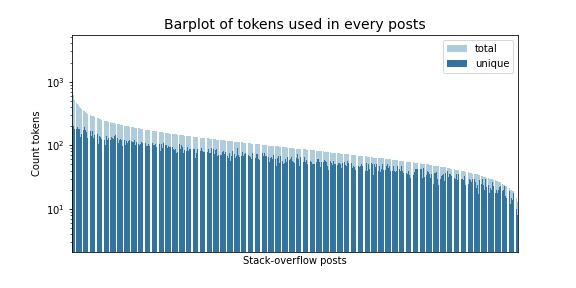
\includegraphics[width=\linewidth]{figures/barplot_tokens1.jpg}
   \end{center}
\end{frame}
%%%%%%%%%%%%%%%%%%%%%%%%%%%%%%%%%%%%%%%%%%%%%%%%%%%%%%%%%%%%%%%%%%%%%%
\begin{frame}{Les données textuelles - Représentation des tokens}
\begin{minipage}{0.48\linewidth}
    \begin{center}
       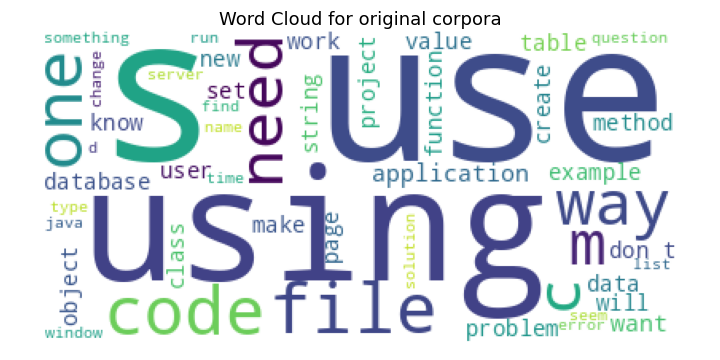
\includegraphics[width=\linewidth]{figures/word_cloud_corpora.png}
    \end{center}
\end{minipage}
\begin{minipage}{0.48\linewidth}
    \begin{center}
       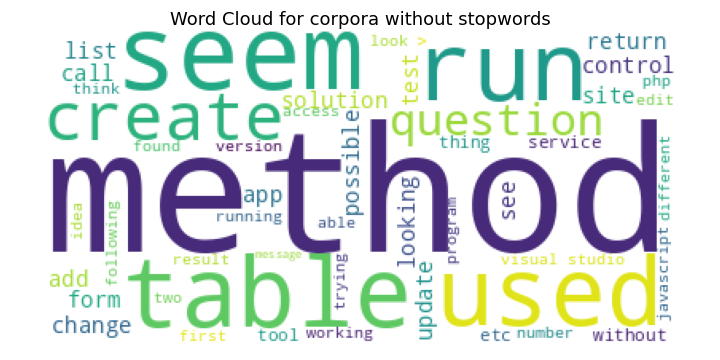
\includegraphics[width=\linewidth]{figures/word_cloud_corpora2.png}
    \end{center}
\end{minipage}
\end{frame}


%%%%%%%%%%%%%%%%%%%%%%%%%%%%%%%%%%%%%%%%%%%%%%%%%%%%%%%%%%%%%%%%%%%%%%
%%%%%%%%%%%%%%%%%%%%%%%%%%%%%%%%%%%%%%%%%%%%%%%%%%%%%%%%%%%%%%%%%%%%%%
\subsection{Exploration sur les tags}
%%%%%%%%%%%%%%%%%%%%%%%%%%%%%%%%%%%%%%%%%%%%%%%%%%%%%%%%%%%%%%%%%%%%%%
%%%%%%%%%%%%%%%%%%%%%%%%%%%%%%%%%%%%%%%%%%%%%%%%%%%%%%%%%%%%%%%%%%%%%%
\begin{frame}{Les tags - Pré-traitements}

\begin{itemize}
    \item \texttt{<c\#><.net><wcf><web-services><soa>}
    \item Filtre nom de langages :\\ \texttt{c$\sharp$, C$\sharp$, c$\sharp$-2.0, c$\sharp$-3.0,  c$\sharp$-4.0 } $\rightarrow$ \texttt{csharp}
    \item Data Frame en one hot encoding 
\end{itemize}
    \begin{center}
       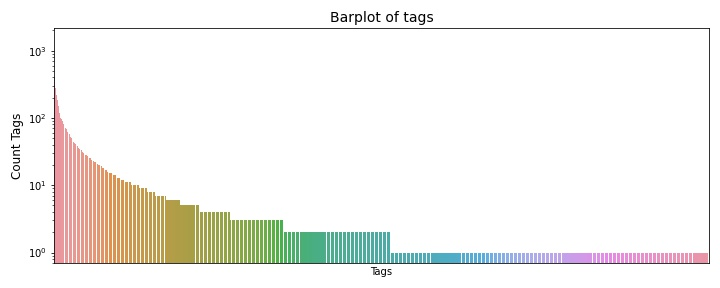
\includegraphics[width=0.9\linewidth]{figures/barplot_tags2.jpg}
    \end{center}
\end{frame}

%%%%%%%%%%%%%%%%%%%%%%%%%%%%%%%%%%%%%%%%%%%%%%%%%%%%%%%%%%%%%%%%%%%%%%
%%%%%%%%%%%%%%%%%%%%%%%%%%%%%%%%%%%%%%%%%%%%%%%%%%%%%%%%%%%%%%%%%%%%%%
\subsubsection*{Réduction de dimension - NMF}
%%%%%%%%%%%%%%%%%%%%%%%%%%%%%%%%%%%%%%%%%%%%%%%%%%%%%%%%%%%%%%%%%%%%%%
%%%%%%%%%%%%%%%%%%%%%%%%%%%%%%%%%%%%%%%%%%%%%%%%%%%%%%%%%%%%%%%%%%%%%%
\begin{frame}{Tags - Création d'une variable univariée}
    \begin{center}
       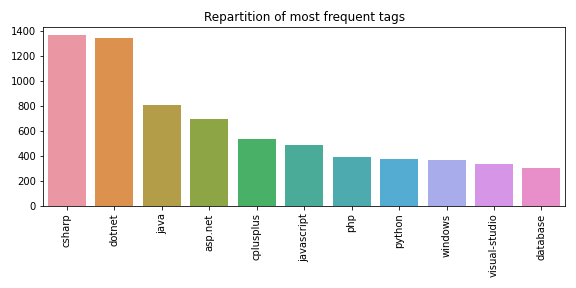
\includegraphics[width=0.9\linewidth]{figures/most_freq_tags.png}
    \end{center}
    $\hookrightarrow$  \texttt{y = tags["csharp"]}
\end{frame}
%%%%%%%%%%%%%%%%%%%%%%%%%%%%%%%%%%%%%%%%%%%%%%%%%%%%%%%%%%%%%%%%%%%%%%
%%%%%%%%%%%%%%%%%%%%%%%%%%%%%%%%%%%%%%%%%%%%%%%%%%%%%%%%%%%%%%%%%%%%%%
\subsubsection*{Réduction de dimension - NMF}
%%%%%%%%%%%%%%%%%%%%%%%%%%%%%%%%%%%%%%%%%%%%%%%%%%%%%%%%%%%%%%%%%%%%%%
%%%%%%%%%%%%%%%%%%%%%%%%%%%%%%%%%%%%%%%%%%%%%%%%%%%%%%%%%%%%%%%%%%%%%%
\begin{frame}{Tags - NMF 1}
La NMF :     
    \begin{center}
        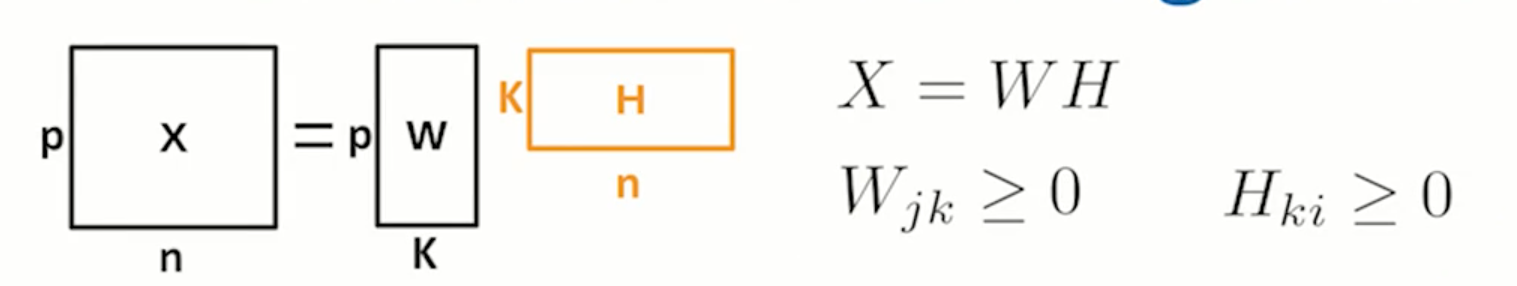
\includegraphics[width=0.9\linewidth]{illustrations/NMF_graphique_explicationOC.png}\\
        {\tiny \color{blue} \href{https://openclassrooms.com/fr/courses/4379436-explorez-vos-donnees-avec-des-algorithmes-non-supervises/4379511-cherchez-les-variables-latentes-qui-expliquent-vos-donnees}{source}}
    \end{center}
Modélisation : 
\begin{itemize}
    \item Sur d'autres tags (\texttt{Id > 10 000}) 
    \item Le choix des hyper-paramètres : 
        \begin{itemize}
            \item Séparation en train - validation
            \item NMF en changeant : \texttt{n\_componants}, \texttt{alpha}, \texttt{l1\_ratio}
            \item Choix des meilleurs paramètres (minimisent le score)
        \end{itemize}
\end{itemize}
\end{frame}
%%%%%%%%%%%%%%%%%%%%%%%%%%%%%%%%%%%%%%%%%%%%%%%%%%%%%%%%%%%%%%%%%%%%%%
\begin{frame}{Tags - NMF 2}
    \begin{center}
      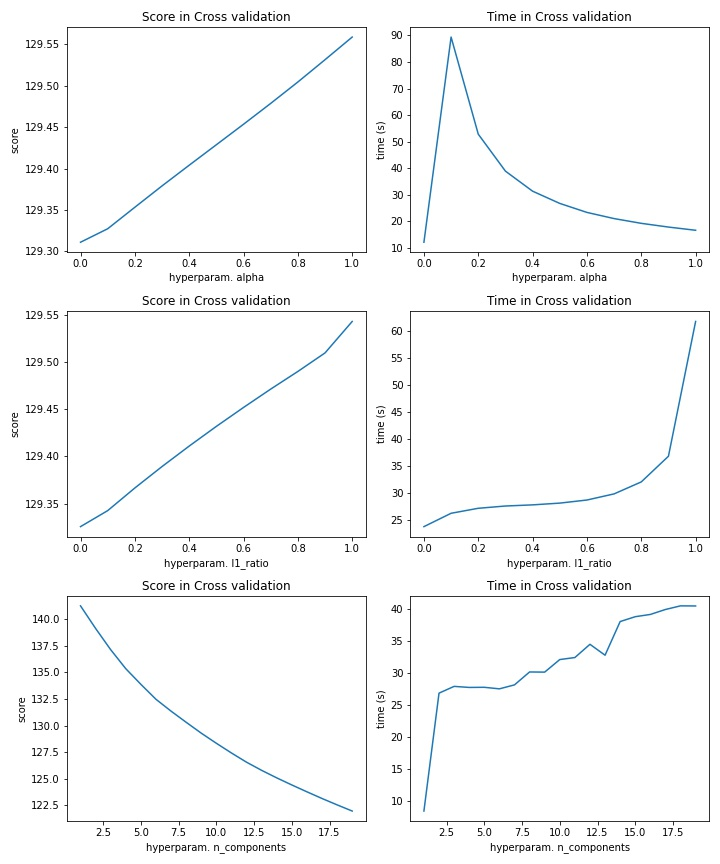
\includegraphics[width=0.6\linewidth]{figures/tags_NMF.jpg}
    \end{center}
\end{frame}
%%%%%%%%%%%%%%%%%%%%%%%%%%%%%%%%%%%%%%%%%%%%%%%%%%%%%%%%%%%%%%%%%%%%%%
\begin{frame}{Tags - NMF 3}
    Les premiers topics de la NMF : 
    \begin{center}
      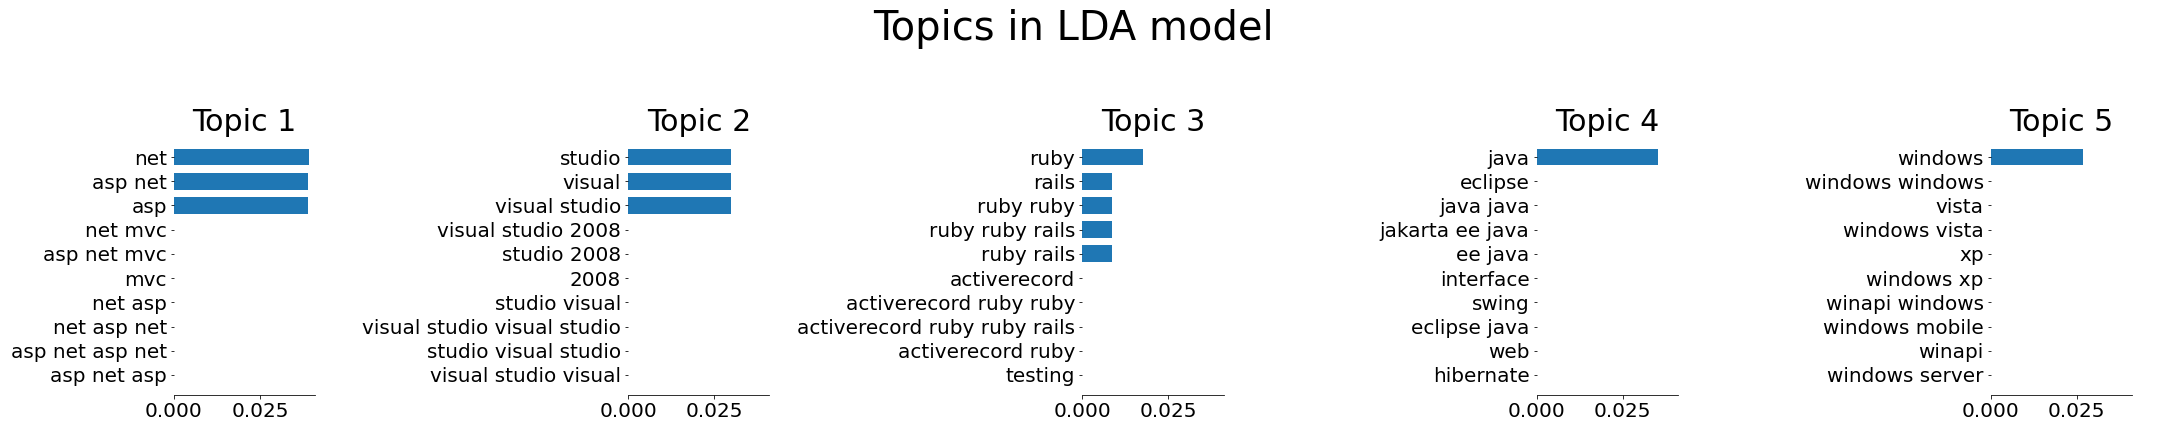
\includegraphics[width=\linewidth]{figures/tags_NMF_topics.png}
    \end{center}\\
    \vspace{0.2cm}
    Projection sur les deux premières composantes : 
    \begin{center}
      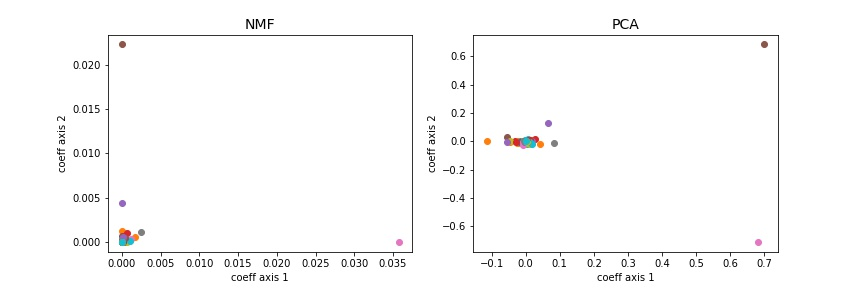
\includegraphics[width=0.9\linewidth]{figures/tags_NMF_PCA_coeffs12.jpg}
    \end{center}
\end{frame}
%%%%%%%%%%%%%%%%%%%%%%%%%%%%%%%%%%%%%%%%%%%%%%%%%%%%%%%%%%%%%%%%%%%%%%
%%%%%%%%%%%%%%%%%%%%%%%%%%%%%%%%%%%%%%%%%%%%%%%%%%%%%%%%%%%%%%%%%%%%%%
\subsubsection*{Réduction de dimension - clustering}
%%%%%%%%%%%%%%%%%%%%%%%%%%%%%%%%%%%%%%%%%%%%%%%%%%%%%%%%%%%%%%%%%%%%%%
%%%%%%%%%%%%%%%%%%%%%%%%%%%%%%%%%%%%%%%%%%%%%%%%%%%%%%%%%%%%%%%%%%%%%%
\begin{frame}{Tags - Clustering hierarchique}
    \begin{center}
       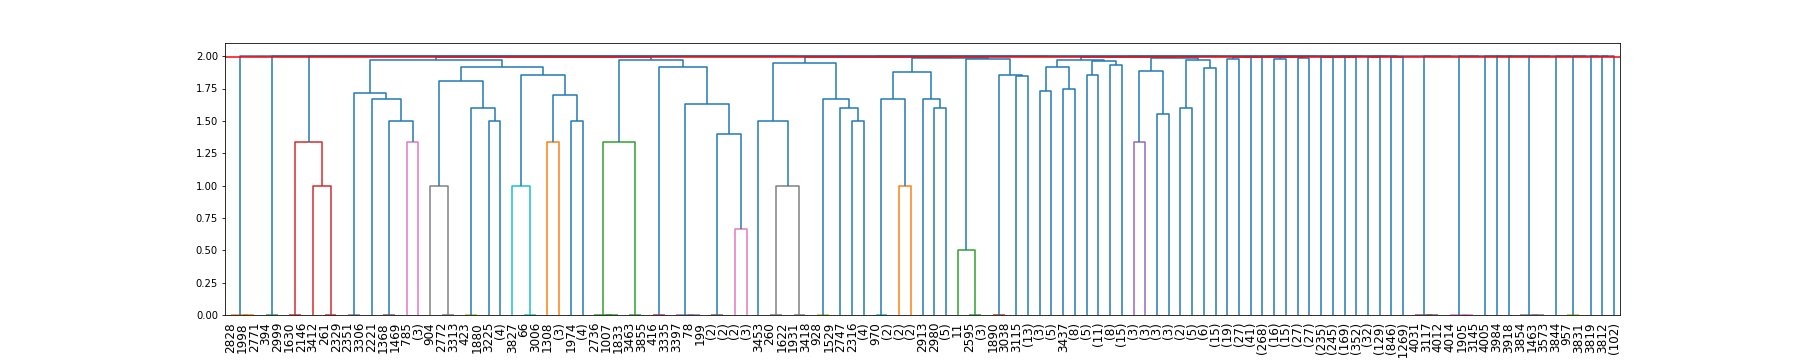
\includegraphics[width=\linewidth]{figures/hierarchical_clustering.png}
    \end{center}\\
    
    $\hookrightarrow$ 12 clusters nommés à partir des tag :\\
    \begin{center}
        {\small \texttt{ linux, language, microsoft, micro\_service, create\_website, python\_website, ruby, tests, python, computer\_architecture, multimedia, object\_oriented }}
    \end{center}
\end{frame}
%%%%%%%%%%%%%%%%%%%%%%%%%%%%%%%%%%%%%%%%%%%%%%%%%%%%%%%%%%%%%%%%%%%%%%
\begin{frame}{Tags - Répartition des clusters}
    \begin{center}
       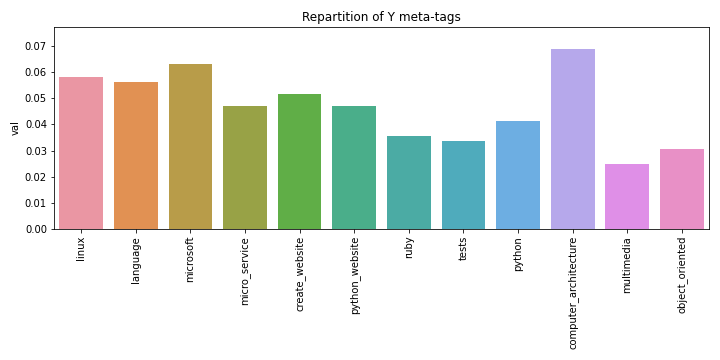
\includegraphics[width=\linewidth]{figures/Y_distribution.png}
    \end{center}
\end{frame}
% %%%%%%%%%%%%%%%%%%%%%%%%%%%%%%%%%%%%%%%%%%%%%%%%%%%%%%%%%%%%%%%%%%%%%%
% \begin{frame}{Produits - nombre de produit commandé}
% \begin{center}
%   \includegraphics[width=0.8\linewidth]{figures/analyse_exploratoire/products_nb_in_orders.jpg}
% \end{center}
% \end{frame}
% %%%%%%%%%%%%%%%%%%%%%%%%%%%%%%%%%%%%%%%%%%%%%%%%%%%%%%%%%%%%%%%%%%%%%%
% \begin{frame}{Produits - nombre d'apparition dans commandes}
% \begin{center}
%   \includegraphics[width=\linewidth]{figures/analyse_exploratoire/products_nb_apperance_log.jpg}
% \end{center}
% \end{frame}
% %%%%%%%%%%%%%%%%%%%%%%%%%%%%%%%%%%%%%%%%%%%%%%%%%%%%%%%%%%%%%%%%%%%%%%
% \begin{frame}{Produits - Réduction nb catégories}
% \begin{itemize}
%     \item Tentative clustering non supervisé
%     \item Séparation par textmining et regroupement si premier mot commun : de $73$ à $49$ catégories
%     \item Recherche information dans les variables numériques pour faire du target encoding : tentative de sélection des catégories avec une régression lasso sur les variables d'ACP\\
% \end{itemize}

% \vspace{0.5cm}
% Pas de structure révélant les catégories mise en évidence. 
% \end{frame}
% %%%%%%%%%%%%%%%%%%%%%%%%%%%%%%%%%%%%%%%%%%%%%%%%%%%%%%%%%%%%%%%%%%%%%%
% \begin{frame}{Produits - Extraction des variables}
% \begin{center}
%   \includegraphics[width=0.6\linewidth]{capture_ecran/product_dtypes.png}
% \end{center}
% \end{frame}

%%%%%%%%%%%%%%%%%%%%%%%%%%%%%%%%%%%%%%%%%%%%%%%%%%%%%%%%%%%%%%%%%%%%%%
%%%%%%%%%%%%%%%%%%%%%%%%%%%%%%%%%%%%%%%%%%%%%%%%%%%%%%%%%%%%%%%%%%%%%%
%%%%%%%%%%%%%%%%%%%%%%%%%%%%%%%%%%%%%%%%%%%%%%%%%%%%%%%%%%%%%%%%%%%%%%
\section{Classification Non Supervisée}
%%%%%%%%%%%%%%%%%%%%%%%%%%%%%%%%%%%%%%%%%%%%%%%%%%%%%%%%%%%%%%%%%%%%%%
%%%%%%%%%%%%%%%%%%%%%%%%%%%%%%%%%%%%%%%%%%%%%%%%%%%%%%%%%%%%%%%%%%%%%%
%%%%%%%%%%%%%%%%%%%%%%%%%%%%%%%%%%%%%%%%%%%%%%%%%%%%%%%%%%%%%%%%%%%%%%
\begin{frame}{LDA et NMF}
    \begin{minipage}{0.48\linewidth}
        NMF : 
        $$ \boxed{ X = W \times H }$$
        \vfill
    \end{minipage}
    \begin{minipage}{0.48\linewidth}
        LDA : 
        \begin{center}
           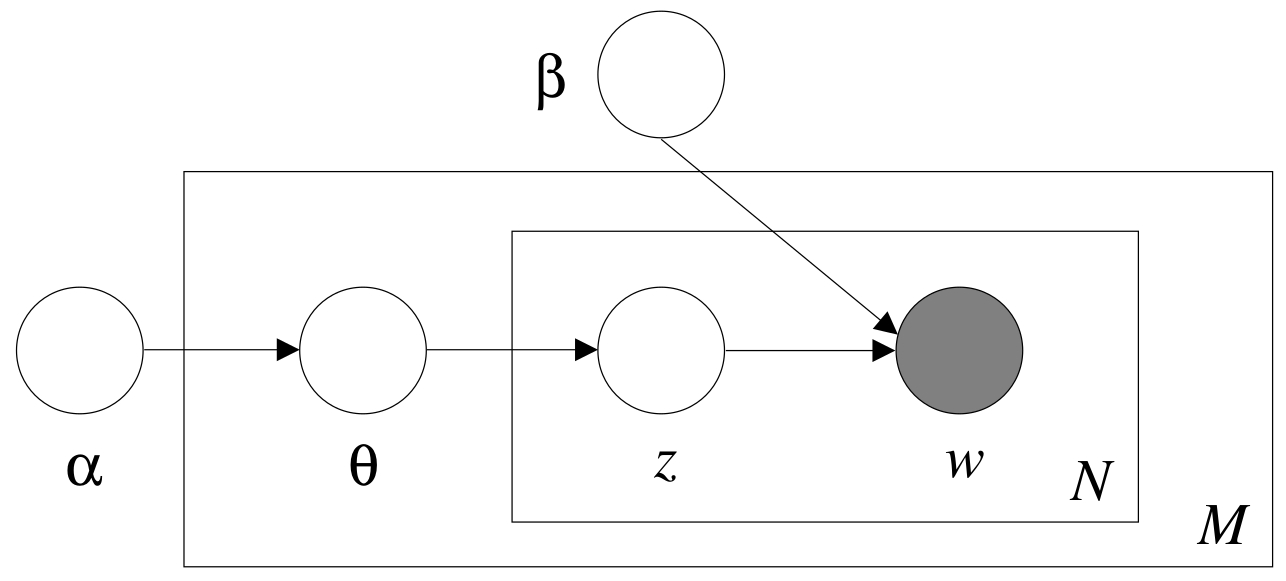
\includegraphics[width=0.8\linewidth]{illustrations/PGM_LDA_original.png}
        \end{center}        
    \end{minipage}
    Résulats de la NMF : 
    \begin{center}
       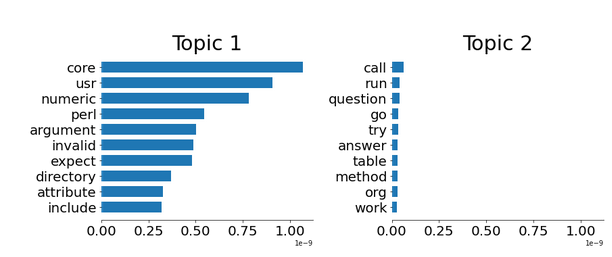
\includegraphics[width=0.8\linewidth]{illustrations/coprus_NMF_topics2.png}
    \end{center}           
\end{frame}
%%%%%%%%%%%%%%%%%%%%%%%%%%%%%%%%%%%%%%%%%%%%%%%%%%%%%%%%%%%%%%%%%%%%
\begin{frame}{LDA sur le corpus}
    \begin{center}
       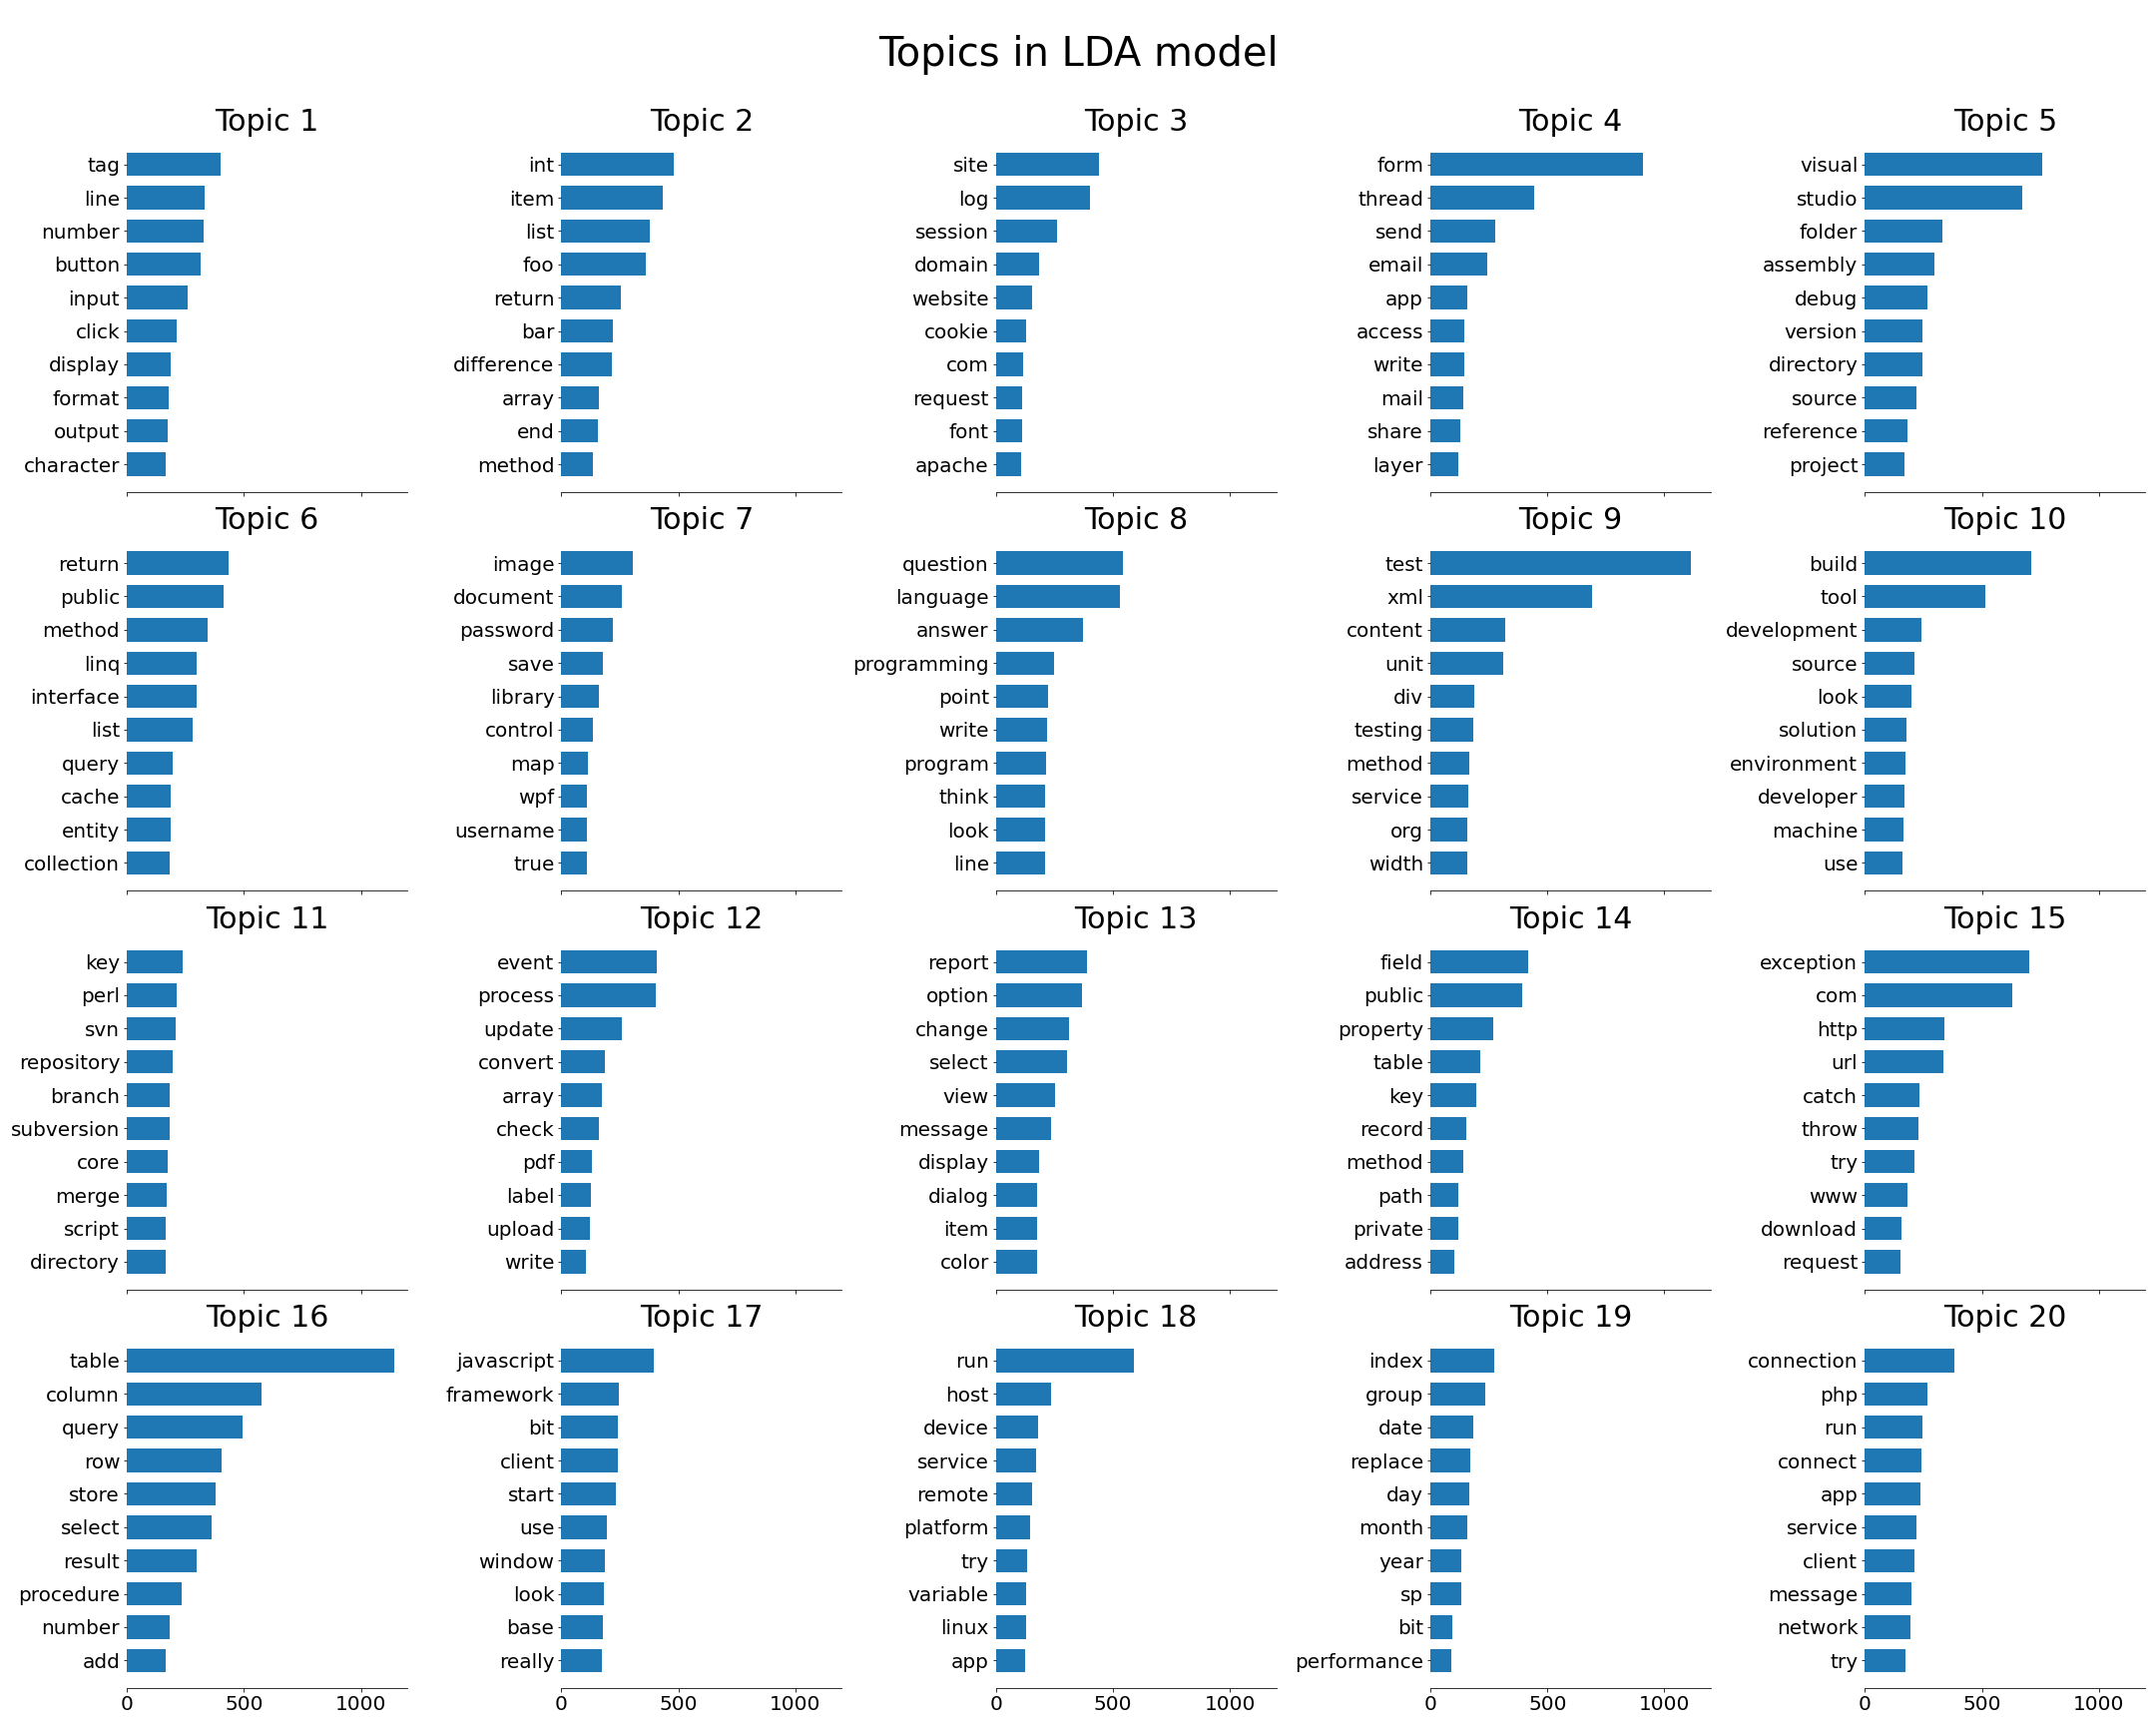
\includegraphics[width=0.9\linewidth]{figures/coprus_LDA_small_topics.png}
    \end{center}
\end{frame}
%%%%%%%%%%%%%%%%%%%%%%%%%%%%%%%%%%%%%%%%%%%%%%%%%%%%%%%%%%%%%%%%%%%%
\begin{frame}{LDA sur le corpus}
    \begin{center}
       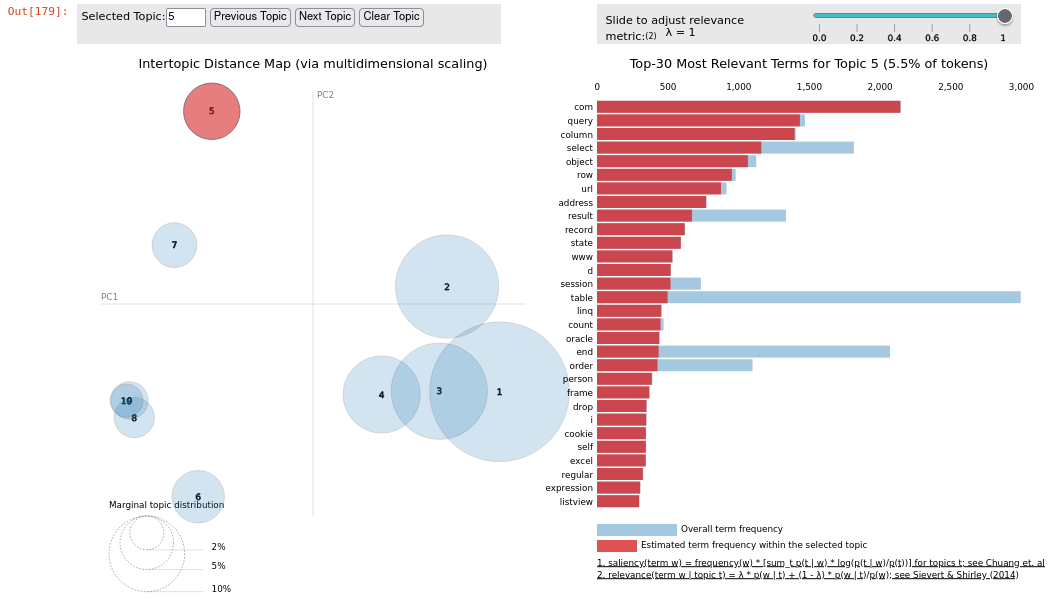
\includegraphics[width=\linewidth]{illustrations/pyLDAviz_topic5_web.png}
    \end{center}
\end{frame}
% %%%%%%%%%%%%%%%%%%%%%%%%%%%%%%%%%%%%%%%%%%%%%%%%%%%%%%%%%%%%%%%%%%%%
% \begin{frame}{Commandes - Dates}
% \begin{center}
%   \includegraphics[width=0.85\linewidth]{figures/analyse_exploratoire/order_time.jpg}
% \end{center}
% \end{frame}

%%%%%%%%%%%%%%%%%%%%%%%%%%%%%%%%%%%%%%%%%%%%%%%%%%%%%%%%%%%%%%%%%%%%%%
%%%%%%%%%%%%%%%%%%%%%%%%%%%%%%%%%%%%%%%%%%%%%%%%%%%%%%%%%%%%%%%%%%%%%%
%%%%%%%%%%%%%%%%%%%%%%%%%%%%%%%%%%%%%%%%%%%%%%%%%%%%%%%%%%%%%%%%%%%%%%
\section{Classification Supervisée}
%%%%%%%%%%%%%%%%%%%%%%%%%%%%%%%%%%%%%%%%%%%%%%%%%%%%%%%%%%%%%%%%%%%%%%
%%%%%%%%%%%%%%%%%%%%%%%%%%%%%%%%%%%%%%%%%%%%%%%%%%%%%%%%%%%%%%%%%%%%%%
%%%%%%%%%%%%%%%%%%%%%%%%%%%%%%%%%%%%%%%%%%%%%%%%%%%%%%%%%%%%%%%%%%%%%%
\subsection{Modèles de classification}
%%%%%%%%%%%%%%%%%%%%%%%%%%%%%%%%%%%%%%%%%%%%%%%%%%%%%%%%%%%%%%%%%%%%%%
%%%%%%%%%%%%%%%%%%%%%%%%%%%%%%%%%%%%%%%%%%%%%%%%%%%%%%%%%%%%%%%%%%%%%%
\begin{frame}{Les différents modèles utilisés}
    \begin{itemize}
        \item Naive Bayes : $ P[ A | B ] = \frac{P[ A \cap B ]}{P[ A \cup B ] }$
        \item Gradient Boosting : min(loss logistique) ou min(loss exponentielle)
        \item Random Forest :\\
    \end{itemize}
    \vfill
    
    Les métriques de classification \\
    \vspace{0.2cm}
    \begin{minipage}{0.48\linewidth}
        Classification binaire
        \begin{itemize}
            \item Accuracy : 
            \item Cross-entropy de classification : 
        \end{itemize}
    \end{minipage}
    \vline
    \hfill
    \begin{minipage}{0.48\linewidth}
        Classification multi-classe
        \begin{itemize}
            \item Accuracy : 
            \item Cross-entropy de classification : 
        \end{itemize}
    \end{minipage}
\end{frame}
%%%%%%%%%%%%%%%%%%%%%%%%%%%%%%%%%%%%%%%%%%%%%%%%%%%%%%%%%%%%%%%%%%%%
\begin{frame}{La séparation des données}
    \begin{minipage}{0.35\linewidth}
        \begin{center}
           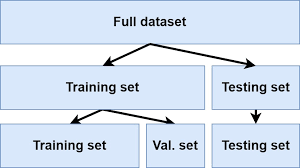
\includegraphics[width=\linewidth]{illustrations/train_test_split.png}
        \end{center}
    \end{minipage}
    \hfill
    \begin{minipage}{0.6\linewidth}
        Séparation des publications
        \begin{itemize}
            \item train/test
            \item Puis train = train/validation par validation croisée\\
            \item Corpus pré-traité
        \end{itemize}\\
    \end{minipage}

    \vspace{0.5cm}
    
    \begin{minipage}{0.48\linewidth}
        Classification binaire
        \begin{itemize}
            \item $y = $ tag le plus courant, $csharp$
            \item Accuracy optimale à 1, à maximiser
        \end{itemize}
    \end{minipage}
    \vline
    \hfill
    \begin{minipage}{0.48\linewidth}
        Classification multi-classe
        \begin{itemize}
            \item $Y = $ méta-tags issus de la classification hiérarchique
            \item Accuracy moyenne, optimale à 1, à maximiser
        \end{itemize}
    \end{minipage}
\end{frame}
%%%%%%%%%%%%%%%%%%%%%%%%%%%%%%%%%%%%%%%%%%%%%%%%%%%%%%%%%%%%%%%%%%%%%%
%%%%%%%%%%%%%%%%%%%%%%%%%%%%%%%%%%%%%%%%%%%%%%%%%%%%%%%%%%%%%%%%%%%%%%
\subsection{Résultats des classifications}
%%%%%%%%%%%%%%%%%%%%%%%%%%%%%%%%%%%%%%%%%%%%%%%%%%%%%%%%%%%%%%%%%%%%%%
%%%%%%%%%%%%%%%%%%%%%%%%%%%%%%%%%%%%%%%%%%%%%%%%%%%%%%%%%%%%%%%%%%%%%%
\begin{frame}{Résultats de la classification binaire :}
    \begin{tabular}{|l|c|c|c|c|}
        \hline
        Modèle & Accuracy & Perte  & Temps & Temps\\
        &  &  & train & predict\\
        \hline
        Aléatoire & 0.25 &  &  &  \\
        CNN LeNet5 & 0.52 & 1.2 & 1min & $<$1s \\
        Transfert VGG16 & 0.82 & 7 & 1min30/cycle & 30s \\
        Transfert ResNet50 & 0.87 & 7 & 1min/cycle& 30s \\
        \hline
    \end{tabular}
\end{frame}
\begin{frame}{Résultats de la classification multi-classe :}
    \begin{tabular}{|l|c|c|c|c|}
        \hline
        Modèle & Accuracy & Perte  & Temps & Temps\\
        &  &  & train & predict\\
        \hline
        Aléatoire & 0.25 &  &  &  \\
        CNN LeNet5 & 0.52 & 1.2 & 1min & $<$1s \\
        Transfert VGG16 & 0.82 & 7 & 1min30/cycle & 30s \\
        Transfert ResNet50 & 0.87 & 7 & 1min/cycle& 30s \\
        \hline
    \end{tabular}
\end{frame}
%%%%%%%%%%%%%%%%%%%%%%%%%%%%%%%%%%%%%%%%%%%%%%%%%%%%%%%%%%%%%%%%%%%%
\begin{frame}{Analyse sur le meilleur modèle et API}
    
\end{frame}
%%%%%%%%%%%%%%%%%%%%%%%%%%%%%%%%%%%%%%%%%%%%%%%%%%%%%%%%%%%%%%%%%%%%%%
%%%%%%%%%%%%%%%%%%%%%%%%%%%%%%%%%%%%%%%%%%%%%%%%%%%%%%%%%%%%%%%%%%%%%%
%%%%%%%%%%%%%%%%%%%%%%%%%%%%%%%%%%%%%%%%%%%%%%%%%%%%%%%%%%%%%%%%%%%%%%
\section{Conclusion}
%%%%%%%%%%%%%%%%%%%%%%%%%%%%%%%%%%%%%%%%%%%%%%%%%%%%%%%%%%%%%%%%%%%%%%
%%%%%%%%%%%%%%%%%%%%%%%%%%%%%%%%%%%%%%%%%%%%%%%%%%%%%%%%%%%%%%%%%%%%%%
%%%%%%%%%%%%%%%%%%%%%%%%%%%%%%%%%%%%%%%%%%%%%%%%%%%%%%%%%%%%%%%%%%%%%%
\begin{frame}{Conclusion}
    Résumé
    \begin{itemize}
        \item Une analyse sur 3 échelles
        \item Deux façons de modéliser le problème
        \item Meilleur modèle = interprétabilité + facilité de calculs
    \end{itemize} 
    \vspace{0.2cm} 
    Améliorations et suite :
    \begin{itemize}
        \item Finir de faire un script avec le meilleur modèle en PEP8
        \item Utiliser la table "orders" pour caractériser les clusters de clients 
    \end{itemize}
    \vspace{0.5cm}
    \begin{center}
        {\Huge Merci pour votre écoute !}
    \end{center}
\end{frame}

\end{document}

